\beginsong{Der Mond ist aufgegangen}[txt={Matthias Claudius, 1778}, mel={Johann Abraham Peter Schulz, 1790}, pfiii={34}, siru={44}, index={Wie ist die Welt so stille}]

\beginverse
\endverse 

\centering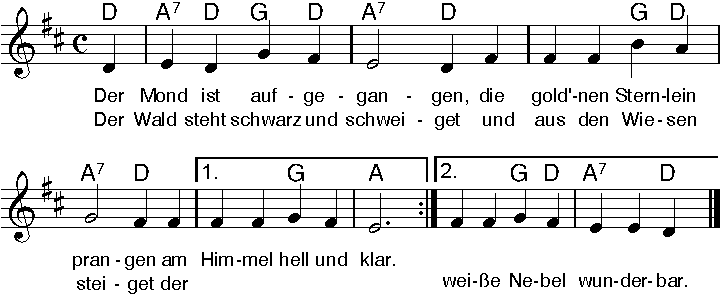
\includegraphics[width=1\textwidth]{Noten/Lied017.pdf}	

\beginverse
\[G]Wie \[D7]ist \[G]die \[C]Welt \[G]so \[D7]stil\[G]le und in der \[C]Dämm'\[G]rung \[D7]Höl\[G]le
so \[G]traulich \[C]und \[G]so \[D]hold! 
\[G]Als \[D7]ei\[G]ne \[C]stil\[G]le \[D7]Kam\[G]mer, wo ihr des \[C]Ta\[G]ges \[D7]Jam\[G]mer
ver\[G]schlafen \[C]und \[G]ver\[D7]gessen \[G]sollt.
\endverse

\beginverse
^Seht ^ihr ^den ^Mond ^dort ^ste^hen? Er ist nur ^halb ^zu ^se^hen
und ^ist doch ^rund ^und ^schön.
^So ^sind ^wohl ^man^che ^Sa^chen, die wir ge^trost ^be^lach^en,
weil ^uns're ^Au^gen ^sie nicht ^seh'n.
\endverse

\beginverse
^Wir ^stol^zen ^Men^schen^kin^der sind eitel ^ar^me ^Sün^der
und ^wissen ^gar ^nicht ^viel.
^Wir ^spin^nen ^Luft^ge^spin^ste und suchen ^vie^le ^Kün^ste
und ^kommen ^wei^ter ^von dem ^Ziel.
\endverse

\beginverse
^Gott, ^lass ^dein ^Heil ^uns ^schau^en, auf nichts Ver^gang^lich's ^trau^en,
nicht ^Eitel^keit ^uns ^freu'n!
^Lass ^uns ^ein^fal^tig ^wer^den, und vor dir ^hier ^auf ^Er^den
wie ^Kinder ^fromm ^und ^fröhlich ^sein!
\endverse

\beginverse
^Wollst ^end^lich ^son^der ^Grä^men aus dieser ^Welt ^uns ^neh^men
durch ^einen ^sanf^ten ^Tod.
^Und ^wenn ^du ^uns ^ge^nom^men, lass uns in ^Him^mel ^kom^men,
du ^unser ^Herr ^und ^unser ^Gott!
\endverse

\beginverse
^So ^legt ^euch ^denn, ^ihr ^Brüder, in Gottes ^Na^men ^nie^der,
kalt ^ist der ^A^bend^hauch.
^Ver^schon' ^uns, ^Gott, ^mit ^Stra^fen und lass uns ^ru^hig ^schla^fen
und ^unser'n ^kran^ken ^Nachbar ^auch!
\endverse

\endsong

\beginscripture{}
Dem Gedicht von Claudius als Vorlage diente "Nun ruhen alle Wälder" (1653) von Paul Gerhardt. Caulius' Todesgedicht vor dem Hintergrund der Heilserwartung eines Christen könnte auch schon vor 1778 in Darmstadt entstanden sein. Seine Einfachheit wurde teilweise als naiv kritisiert, erfreute sich jedoch schnell großer Beliebtheit in der deutschen Bevölkerung.
\endscripture

\begin{intersong}

\end{intersong}